\documentclass[A4]{scrartcl}
\usepackage[english]{babel}
\usepackage{hyperref}
\usepackage{mathtools}
\usepackage{listings}
\usepackage{graphicx}
\usepackage{subcaption}
%\usepackage[ddmmyyyyy]{datetime}

\usepackage[%
  backend=bibtex      % biber or bibtex
%,style=authoryear    % Alphabeticalsch
 ,style=numeric-comp  % numerical-compressed
 ,sorting=none        % no sorting
 ,sortcites=true      % some other example options ...
 ,block=none
 ,indexing=false
 ,citereset=none
 ,isbn=true
 ,url=true
 ,doi=true            % prints doi
 ,natbib=true         % if you need natbib functions
]{biblatex}
\bibliography{bib}



\begin{document}
\title{Graph500 in the public cloud.}
\subtitle{Research Project 2 - Proposal}
\date{\today}
\author{Harm Dermois \\ harm.dermois@os3.nl}

\maketitle
\newpage


\begin{abstract}
\textit{hello Abstract stuff}
\end{abstract}

\newpage

\section*{Acknowledgments}
I would like to thank my supervisor, Ana Varbanescu for her close involvement in this project. I also want to thank Ana Opresecu with the advise and help see provided with working in the cloud.

\tableofcontents
\newpage




\section{Introduction}
\label{sec:introduction}
%TODO ADD some more to this
%Modern HPC applications are optimized to process 3D physics simulation, but are not well suited for data intensive problems.
The Graph 500 \cite{murphy2010introducing} is a list of top 500 graph processing machines. As of late the need for network analysis is skyrocketing. Network analysis includes social networks, road direction and even text analysis. 

The Graph 500 is inspired by the TOP500 \cite{top500}. The TOP500 uses the LINPACK benchmark which solves linear equations and linear least-squares problems. The metrics used in the LINKPACK are useful or CPU intensive problems, but do not quantify the ability to process graphs. For this reason, a new benchmark is made with metrics which better suit data intensive problems. The benchmark was made with the following ideas in mind: the kernel should generic and apply to many applications, the results should map to real world problems and the data set should be comparable to real-world problems. The benchmark is meant to push the industry to invest into building specific hardware to more efficiently tackle these types of problems.


To get on the list, a benchmark should be run. This benchmark needs to comply to some specifications which can be found on the Graph500 website\cite{graph500-specs}, but beyond these specifications anything goes. This means that the benchmark can be optimized for the hardware it runs on. 

The benchmark consists of two kernels: the graph construction and the Breadth-First Search(BFS). Both these kernels will be timed. The kernels are preceded by the creation of an edge-list using a Kronecker Generator\cite{leskovec2010kronecker}. The results of both kernels are validated and the performance information is output.
\\
The Graph500 list, at the moment, consists mostly of super computers. The aim of this project is to get an entry on the Graph500 list using the public cloud. The research focuses on defining a model to make a predict how many machines will be needed to get a certain performance.






\section{Research Question}
\label{research-questions}
%TODO need to changed to better suit the results.
The research question for this project is as follows: \\
Is it possible to make a model that can predict the performance depending on the amount of resources? \\
To answer our main question, the following sub-questions have been formulated: 
\begin{itemize}
\item What size of graph is reasonable to benchmark while working on the cloud?
\item How well does the reference implementation\cite{graph500-code} run on the public cloud?
\item What model fits the results acquired from running the benchmark on the cloud?
\end{itemize}

The research will focus on running the Graph 500 MPI reference implementations. These implementations are created by the owners of the Graph 500 and there is no doubt that the implementations adhere to the specifications. The Graph500 times two kernels: the graph generation and the BFS. The focus of the project will be on the BFS. The BFS performance is the most important metric and is shown on the list.


\section{Related Work}
\label{related-work}
There is a lot of related work on the Graph500 benchmark. Most of these papers focus on the implementation of better BFS kernels and are not applicable for our study.

In a paper, by Chaktranont et al.\cite{chakthranont2014exploring}, the difference is shown between \texttt{graph500\_mpi\_simple} on a virtual private cluster and on a physical cluster. The paper shows that the  virtualization overhead head is about 5\% on the HPC Cloud they created. This is a cloud solution specifically created for super computers. Comparing this with other cloud solutions might give some insights.

Toyotaro Suzumura et al. \cite{suzumura2011performance} investigated the reference Graph 500 implementation. The paper gives detailed explanation of three of the four implementations and provides a performance evaluation of these implementations. They managed to reach 8 GTEPS for a scale 34 problem and provide some insight about how to optimize the algorithms. The implementation used in this project is described and their evaluation and communication model are used.

A technical paper by Angel et al.\cite{angel2012graph} runs the Graph500 simple implementation on UMBC High Performance Computing Facility. In this paper the simple implementation runs on their cluster up to scale 32 and 64 nodes. They share a way of removing the validation from the program. The experiments are done by running multiple instances of the program on the same node for up to 64 nodes and explain the implication of running the program in such a way. The hardware used is similar to the DAS-4. They also propose a way to turn off validation, which is also used in our project.

To summarize, there has been a lot of work done on performing and optimizing the Graph 500 benchmark, but to our knowledge no one has attempted to run the Graph 500 benchmark on a public cloud yet.


\section{Scope}
\label{scope}
The research will focus on running the MPI Graph500 reference implementation. The other benchmarks will not be considered. Optimization will only be done for running the implementation on the cloud.
The main focus of the project will be on the amount of edges that will be traversed. The generation of the graph will have a less prominent role.

\section{Background}
\label{background}
This section contains information needed to understand the project and the work related to this project.

%\subsection{Kronecker graph}
%The graph that is used by the Graph500 is the Kronecker graph\cite{leskovec2010kronecker}. This is because a Kronecker graph has some nice properties which are also seen in graph that can be seen in the real world.
%TODO list of properties which are important to the graph500.
%TODO Say something about the properties of the graph. is a tree, so undirected.



\subsection{Graph500 Benchmark 1 ("Search")}
Benchmark 1 ("Search")\cite{graph500-specs} consists out of two kernels accessing a single data structure representing an undirected graph. These kernels are: the construction of the graph from the a list of tuples and a search through the constructed graph. 

The benchmark has defined a few different problem classes. These are shown in table \ref{tab:problem_scales}. 
\begin{table}[!h]
	\begin{center}
	\begin{tabular}{|l|l|l|l|}
		\hline
		Problem class     & Scale & Edge Factor & Approx. Storage size in TB \\ \hline
		Toy (level 10)    & 26    & 16          & 0.0172                     \\ \hline
		Mini (level 11)   & 29    & 16          & 0.1374                     \\ \hline
		Small (level 12)  & 32    & 16          & 1.0995                     \\ \hline
		Medium (level 13) & 36    & 16          & 17.5922                    \\ \hline
		Large (level 14)  & 39    & 16          & 140.7375                   \\ \hline
		Huge (level 15)   & 42    & 16          & 1125.8999                  \\ \hline
	\end{tabular}
	\caption{The lists of problem classes as defined by the Graph 500, assuming the storage of the edge list is done n a 64-bit integer.}
	\label{tab:problem_scales}
	\end{center}
\end{table}
These problem classes give a sense of the size of the  and the amount of storage which is needed to run the experiment. The scale is defined as a combination of the amount of vertices and the edges connected to each of these vertices($2^{scale} * edgefactor = number of edges$). The number of vertices is given by the variable scale. In the case of the Toy  problem it is $2^26$ vertices in the graph. The other parameter is the edge factor is the amount of edges which is connected the graph. In each of the problem classes used by the Graph500 an edge factor of 16 is used. In this project the same number will be used for each of the experiments and the scale will be variable.

The benchmark consists of the following steps:
\begin{enumerate}
	\item Generate the edge list.
	\item Construct a graph from the edge list.
	\item Randomly sample 64 unique search keys.
	\item For each search key:
	\begin{enumerate}
		\item Create an array with all nodes up till the key.
		\item Validate that the parent array is a correct BFS search tree for the given search tree.
	\end{enumerate}
	\item Compute the performance
\end{enumerate}
In the following subsections the all the steps of the benchmark are explained in more detail.

\subsubsection{Generating the edge list}
First off the edge list needs to be generated. 
%TODO needs to be edited
The data generator constructs a list of edge tuples containing vertex identifiers, but also contains the start and end vertex. Each edge in the list is undirected.

The intent of the graph generation is to convert a the edge list, which has no locality, into a data structure which can more easily be used. The list of generated tuples could have some locality because of the way the edges are generated. To lose this possible locality the generated edges are randomized before inserted in to the graph generation kernel. 

The graph generated is a Kronecker graph which has many properties which are seen in graphs in the real world, see reference \cite{leskovec2010kronecker}.

\subsubsection{Graph Construction}
The graph construction is the first kernel. This kernel is timed for the benchmark. The kernel takes the previously created edge list and may transform it in any desired of data structure, a few examples of such data structures are Compressed Row Storage(CRS) and Compressed Sparse Column. These two data structures will be explained in more detail in the next section. The kernel takes only two parameters, the edge list and the size of the edge list. The number of vertices and other information that might be inferred from the edge list must be done computed by the kernel. 

One thing to note is that the data structure created in this kernel cannot be altered by subsequent kernels. 

\subsubsection{Sampling 64 search keys}
After the graph is constructed a few searches need to be done. By performing these searches the speed of traversal can be measured. The search keys needs to have at least one other vertex connected to them. The search is done in a Breadth First Search way.

\subsubsection{Breadth First Search}
Breadth First Search\cite{bfs} (BFS) is the way of traversing a graph chosen by the Graph 500. BFS visits all vertices each on the level before moving on to the next level. The level of a vertex is defined as the minimum number of edges that need to traversed to get ot the root. It keeps traversing the Graph 500 until all vertices in the graph have been visited. An example of the traversal can be seen in figure \ref{fig:bfs}. If the search key is H then the output of the BFS will be A-H in alphabetical order.
Note that the benchmark  BFS  specifies the end results, but does not specify how the program gets to this result.
\begin{figure}[!h]
	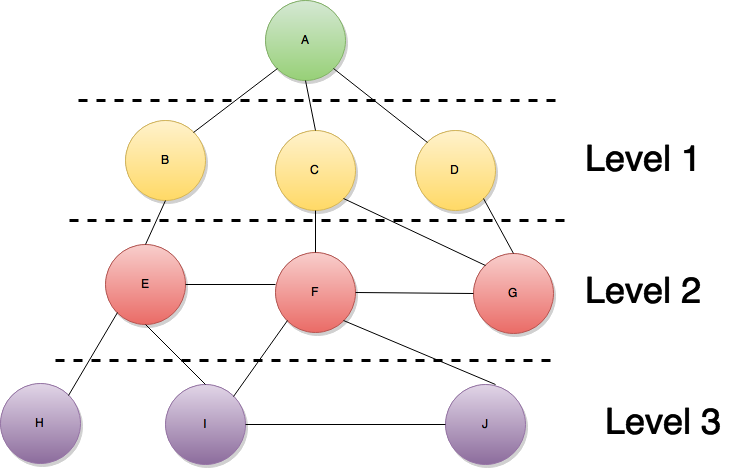
\includegraphics[width=\textwidth]{images/BFS-example1-with-levels}
	\caption{An example of BFS traversal is shown here. The nodes are traversed in alphabetical order.}
	\label{fig:bfs}
\end{figure}

\subsubsection{Validation}
After the each of the searches a validation is done. The validation does soft checking of the result, because there is some randomness in the process, which makes validating it against a reference hard. This validation checks for the following things:
\begin{enumerate}
\item The BFS tree is a tree and does not contain cycles.
\item Each tree edge connects vertices whose BFS levels differ by exactly one.
\item Every edge in the input list has vertices with levels that differ by at most one or that both are not in the BFS tree.
\item The BFS tree spans an entire connected component's vertices.
\item A node and its parent are joined by an edge of the original graph.
\end{enumerate}


\subsubsection{Timing and Performance metrics}
The output should at least contain these measurements. \\ 
%TODO needs to be edited taken from graph500 Need to add the step in more detail.
\textbf{Timing} \\
Start the time for a search immediately prior to visiting the search root. Stop the time for that search when the output has been written to memory. Do not time any I/O outside of the search routine. If your algorithm relies on problem-specific data structures (by our definition, these are informed by vertex degree), you must include the setup time for such structures in each search. The spirit of the benchmark is to gauge the performance of a single search. We run many searches in order to compute means and variances, not to amortize data structure setup time.


In order to compare the performance of Graph 500 "Search" implementations across a variety of architectures, programming models, and productivity languages and frameworks, we adopt a new performance metric described in this section. In the spirit of well-known computing rates floating-point operations per second (flops) measured by the LINPACK benchmark and global updates per second (GUPs) measured by the HPCC RandomAccess benchmark, we define a new rate called traversed edges per second (TEPS). We measure TEPS through the benchmarking of kernel 2 as follows. Let timeK2(n) be the measured execution time for kernel 2. Let m be the number of input edge tuples within the component traversed by the search, counting any multiple edges and self-loops. We define the normalized performance rate (number of edge traversals per second) as:
\\
$TEPS(n) = m / timeK2(n)$
\begin{description}
\item[SCALE] Graph generation parameter
\item[edgefactor] Graph generation parameter
\item[NBFS] Number of BFS searches run, 64 for non-trivial graphs
\item[construction time] The single kernel 1 time
\item[min time, firstquartile time, median time, thirdquartile time, max time] Quartiles for the kernel 2 times
\item[mean time, stddev time] Mean and standard deviation of the kernel 2 times
\item[min nedge, firstquartile nedge, median nedge, thirdquartile nedge, max nedge] Quartiles for the number of input edges visited by kernel 2, see TEPS section above.
\item[mean nedge, stddev nedge] Mean and standard deviation of the number of input edges visited by kernel 2, see TEPS section above.
\item[min TEPS, firstquartile TEPS, median TEPS, thirdquartile TEPS, max TEPS]  Quartiles for the kernel 2 TEPS
\item[harmonic mean TEPS, harmonic stddev TEPS] Mean and standard deviation of the kernel 2 TEPS. Note: Because TEPS is a rate, the rates are compared using harmonic means.
\end{description}

\begin{lstlisting}
SCALE:                          24
edgefactor:                     16
NBFS:                           64
graph_generation:               16.2365
num_mpi_processes:              8
construction_time:              15.4957
min_time:                       13.9349
firstquartile_time:             15.6177
median_time:                    15.7516
thirdquartile_time:             15.8136
max_time:                       16.1873
mean_time:                      15.6812
stddev_time:                    0.318657
min_nedge:                      268435456
firstquartile_nedge:            268435456
median_nedge:                   268435456
thirdquartile_nedge:            268435456
max_nedge:                      268435456
mean_nedge:                     268435456
stddev_nedge:                   0
min_TEPS:                       1.65831e+07
firstquartile_TEPS:             1.6975e+07
median_TEPS:                    1.70418e+07
thirdquartile_TEPS:             1.71879e+07
max_TEPS:                       1.92635e+07
harmonic_mean_TEPS:             1.71183e+07
harmonic_stddev_TEPS:           43826.4
Program time:                    1035.57
\end{lstlisting}


\subsection{Graph compression}
\label{back:compression}
The graphs used in the benchmark are 


\subsection{Reference Implementations}

%TODO detailed explanation about the algorithm how the division is done between the node. Layers. Need to be edited alot Combined to different pieces
The version used in this project is version 2.1.4\cite{graph500-code}. In this version there are four different implementations MPI implementations which all parallelization in the same way. The names of these implementations are: simple, one sided, replicated and replicated csc. All graphs use some form of storing the sparse graph in a compressed form explained as mentioned in the previous section. The one sided implementation is not be considered, because the one sided implementation expects high performance remote memory access to work properly. This is a technique which can not be relied on in the public cloud, because you have no control over the environment. This is why it is better to stick to the basics. 


%TODO this is more detailed.
As mentioned in the section \ref{related-work} the reference implementations have been studied in detail. The reference which will be used in this project is the  simple one. This has been chosen because it is the most simple to understand, has been thoroughly studied and requires the least amount of RAM on each of the nodes. The decision made to run everything on the RAM was done, because this is easier to implement no shared file system was needed. 

Here a brief description of the algorithm will be given a more detailed explanation can be found in the by Suzumara et al.\cite{suzumura2011performance}.
 
The implementation uses 2 queues for the BFS. The first queue is used to store all nodes that should still be visited in this iteration. The second queue is used to store all the nodes that should be visited in the next iteration. When the first queue is empty the roles will be swapped of the queues and the next iteration will start. This is done until there are no more nodes that should be visited.
After each level a synchronization is done before the next level can begin. 
%The synchronization is needed because otherwise nodes from the wrong level can be put in the wrong queue.

The nodes are evenly distributed between the processes. This is done by looking at the rank of the process and the modulo of the number of processes to divide them.

The graph is stored in a CSR way to minimize the amount of data that needs to be stored in the ram.

The paper that was previously mentioned also gives an estimate of the amount of communication in the simple algorithm. The formula is:\\
\begin{equation}
\label{eq:communication_size}
C(n, M) = A * B * C * D (bytes).
\end{equation}
Where $A = M*2, B = (n-1)/n, C=2, and D=8$ \\

For example, if s $=$ 32 and n $=$ 128 (128 MPI processes), then the total communication 
data volume $C(128, M)$ is calculated as $2^{32}$ $*$ 16 $*$ 2 $*$ $(127/128)$ $*$ 2 $*$ 8 = 2032 GB (2 TB). As previously noted, the entire graph for M(32) was 
1.03 TB, so the amount of data was doubled.

\section{Methodology}
\label{methodology}
Introduction to the methodology.

\subsection{Experiments}
This section contains an explanation explains which experiments have done and which parameters were used.
%TODO Write something about using the Maximum value of the TEPS for each of the graphs.Results or in the Experiments.
\subsubsection{Problem scale and Edge Factor}
The Graph500 has defined a few different problem scales these can be seen below in table \ref{tab:problem_scales}. 
\begin{table}[!h]
\begin{tabular}{|l|l|l|l|}
\hline
Problem class & Scale & Edge Factor & Approx. Storage size in TB\\ \hline
Toy (level 10) &	26 &	16 &	0.0172\\ \hline
Mini (level 11) &	29 &	16 &	0.1374\\ \hline
Small (level 12) &	32 &	16 &	1.0995\\ \hline
Medium (level 13)& 	36 &	16 &	17.5922\\ \hline
Large (level 14) &	39 &	16 &	140.7375\\ \hline
Huge (level 15) &	42 &	16 &	1125.8999\\ \hline
\end{tabular}
\caption{The lists of problem classes as defined by the graph500}
\label{tab:problem_scales}
\end{table}
These problem classes give a sense of the size of the problem and the amount of storage which is needed to run the experiment. The scale is defined as a combination of the amount of vertices and the edges connected to each of these vertices($2^{scale} * edgefactor = number of edges$). The number of vertices is given by the variable scale. In the case of the Toy  problem it is $2^26$ vertices in the graph. The other parameter is the edge factor is the amount of edges which is connected the graph. In each of the problem classes used by the Graph500 an edge factor of 16 is used. In this project the same number will be used for each of the experiments and the scale will be variable. 

%Because this project deals with commodity hardware we have more freedom in the virtual hardware that will be used. The baseline needs to be adjusted to the variety which is available. For this the amount of experiments will be very varied, but the problem scale should not be to large. Therefore the project will focus on the TOY and mini problem classes. This means a scale of 26 and 29. If the resources allow the small problem scale will also be considered.



\subsection{Measurements}
The measurements are run for the scale 9,12,15,21,24 and 30(30 in some cases) on 2,4,6,16 and 32(in some cases) nodes. Each node will only contain 1 process. The platforms on which the measurements will be done are: DAS-4, OpenNebula and Amazon Webservices.

\subsection{OpenMP}
The reference  implementation has also implemented some loops using OpenMP. To find out what the effect is of OpenMP on the TEPS, only one node was used and assigning different amount of CPUs to be used. By default OpenMP will decide itself how many nodes will be the best to use for the problem at hand. By specifying the amount of CPUs the influence of OpenMP on the results can be measured. To do the OpenMP experiments a small change needed to be made in the code to turn off the dynamic assignment and assign the number of CPUs that should be used. The experiments were done one node of the LU cluster. The experiments were only done for a limited number of scale, because at larger scale the experiment could not run on one node. Validation was still turned on for these experiments.

\subsection{MPI}
The Graph500 simple implementation can only run with a number of nodes which is a power of 2. This constraint limited the amount of experiments that could be done. the As seen in section \ref{hw:das4} and \ref{hw:opennebula} there can be experiments done with up to 16 nodes on the LU and up to 32 nodes on the VU. In principle experiments could be done with 62 nodes on the VU, but some of the nodes were out of service and there is always someone else using one of the nodes which makes it hard to run an experiment with 64 nodes.
The experiments will be done on the DAS-4 and OpenNebula as a reference for the experiments on the commercial cloud. These experiments will also be used to see if any model can be made to predict the amount of lines that will be traversed given a scale an amount of nodes. Note that the simple algorithm only allows for node amounts which are a power of 2. Multiple different experiments were done for the MPI. The following types experiments were done:
\begin{itemize}
	\item With validation, the simple implementation without any modifications.
	\item Without validation, the simple implementation without validation.
	\item Without Infiniband
	\item On the OpenNebula
	\item Amazon C3 type
	\item Amazon R3
\end{itemize}



    
\subsection{Communication}
\label{med:comm}
%Needs to be revised and more  precise.
To confirm that the model used for the communication is sound messages have logged each time a MPI message is send. There are 3 types of messages sent in this program. The type of message is a message send when the buffer is full. When process buffer is full it will sent the message to the recipient. The buffer has was fixed (2 kB) in each of the experiments but it can be changed to get better performance. The second type of message flushing the buffer. If all nodes have been visited by the program and the buffer still has some nodes that need to be visited it will flush the buffer and share the remaining nodes that need to be visited. The last message is used to report that the program is completely done. The process sends an empty message to other programs stating it is done.

Also the IMB benchmark will be done for each of the environments to measure the time it takes to send messages. The benchmark consists of multiple modules. The modules that are interesting for the project is the PingPong. 

\subsection{Memory consumption}
%TODO needs to edited This needs to be paired with the 
Since the Graph500 organization provides different reference implementations with different formats, the amount of data differs. However, with the sparse matrix format called CSR (Compressed Sparse Row), the memory consumption is $E*2 + V (E = \# of edges, V = \# of vertices)$.
$M(Scale) = (2^{Scale} *(2*edgefactor + 1))$. The E here is calculated as the product of V by the edgefactor, which is 16 in this benchmark. For
example, $M(32) = 2^{32} * (2*16+1) * 8 (bytes) = 1.03125 TB$.
\begin{table} [!h]
\begin{tabular}{|l|l|l|}
\hline
scale & 2 Nodes& 4 Nodes \\ \hline
9 & 0.000067584	&	0.000033792 \\ \hline
12 & 0.000540672	&	0.000270336\\ \hline
15 & 0.004325376	&	0.002162688\\ \hline
18 & 0.034603008	&	0.017301504\\ \hline
21 & 0.276824064	&	0.138412032\\ \hline
24 & 2.214592512	&	1.107296256\\ \hline
27 & 17.716740096	&	8.858370048\\ \hline
30 & 141.733920768	&	70.866960384\\ \hline


\end{tabular}
\caption{This table shows a few calculations for how much memory is consumed with 2 and 4 nodes. To continue the table for mode nodes the values need to be divided by 2. For higher scales the formula previously mentioned should be used. Calculated memory consumption. This needs to be doubled because you also store the parent.}
\label{tab:calculation memory consumption}
\end{table}
    
\subsection{Amazon}
For experiments on AWS a new HVM image was created, which is similar to the VM used on OpenNebula. The base of this image is (ami-15011a61) a public image which also has the 5.x version of CentOS. On this image keys were placed, MPI installed and the git repository downloaded. There is one thing changed in the way the experiment is performed on the DAS and OpenNebula. The \texttt{mpirun} command is started from one of the nodes instead of from a node which does not participate in the calculation. This is done setting up an \texttt{SSH} connection to the server and then running the command remotely, for the command see Appendix [REF to used commands]. Running MPI in this manner might have some influence on the performance of that one node.
\subsection{Tools}
\subsubsection{MPI and OPENMP}

\subsubsection{Intel MPI Benchmark}
Intel MPI Benchmark(IMB) was used to get find out how well MPI performs in the setup. This is a free benchmark that can be used to measure the MPI functions on specific setups. The program was compiled using the OpenMPI compiler, details of the compilation can be found in Appendix [reference compilation benchmark].

\subsection{Hardware}
The goal of the project to do a Graph500 benchmark on the cloud and find out a model to predict the performance of the benchmark. For this a experiments were done on the DAS-4 to create a baseline. In the following sections the hardware used will be shown.
\subsubsection{Das-4}
\label{hw:das4}
The Distributed ASCI Supercomputer 4 (DAS) is a six-cluster wide-area distributed system designed by the Advanced School for Computing and Imagining (ASCI)\cite{das-4}. The six-clusters are the following:
\begin{itemize}
\item Vrije Univeristeit (VU)
\item Leiden Univeristeit (LU)
\item Univeristeit van Amsterdam (UvA) 
\item Technische Universiteit Delft (TUD)
\item Univeristeit van Amsterdam - The MultimediaN (UVA-MN) 
\item Astronomy institute Netherlands Institute for Radio Astronomy (ASTRON)
\end{itemize}
All computations have been done on the clusters from he VU and LU. These two clusters were chose because the cluster of LU is not actively in use and has the nodes with the most memory. The VU cluster was used, because it has the most machine available and has an OpenNebula cluster installed on it. The specifications of the clusters can be found in table \ref{tab:das-clusters}. 

Each of the nodes in the clusters has a dual quad-core processor with a speed of 2.4 GHz. All the nodes all also connected with InfiniBand\cite{infiniband}.
\begin{table}[!h]
\begin{tabular}{|l|l|l|}
\hline
Cluster & Number of nodes  & Memory(GB) \\ \hline
VU 		& 74 (41) for all purposed	 & 24			\\ \hline
LU		& 16 & 48 \\ \hline
\end{tabular}
\caption{The specifications of the clusters used in this project.}
\label{tab:das-clusters}
\end{table}
All nodes on the cluster have CentOS release 6.6 (Final) installed on them.


\subsubsection{OpenNebula}
\label{hw:opennebula}
``OpenNebula  provides the most simple but feature-rich and flexible solution for the comprehensive management of virtualized data centers to enable private, public and hybrid IaaS clouds. OpenNebula interoperability makes cloud an evolution by leveraging existing IT assets, protecting your investments, and avoiding vendor lock-in.''\cite{opennebula}. The version of OpenNebula(ON) installed on the VU cluster is version 3.8. The ON cluster used consisted of 8 nodes with the following specs: $400 / 2400 (16\%)  39.1G / 63G (61\%)$. For the experiments the following two templates were used seen in Appendix[Reference].

For the experiments using 2 to 16 nodes each of the VMs got a 24 GB of memory. This amount has been chosen because this is the same amount as the nodes on the VU cluster. For the experiment with 32 VMs the nodes have only 10 GB. 10GB was chosen because the 8 nodes could not handle 32 nodes with the same specification as used for experiments before. With this setup the experiments could still be run, because the graph is distributed between the nodes. 

The VMs used for the ON experiments have CentOS release 5.11 (Final) installed. The version of MPI was 1.4. On the VMs no InfiniBand has been installed. 


\subsection{Reference Implementation}


\section{Results}
\label{results}
In this section the results will be shown for this project.

\subsection{OpenMP}
\label{sec:openmp}
As mentioned in [ref to tools] OpenMP can be used to parallelize loops and other easy functions that can be easy to make parallel. Figure \ref{fig:graph_generation} shows a graph of the amount of time spent generating the graph as a function of the amount of cores that were assigned to the program. The figure shows that the time spent is  dependent on the amount of CPUs. Each time the amount of CPUs doubles the time spent is halved. 
 % These experiments have been on the DAS with validation on.

\begin{figure}[!h]
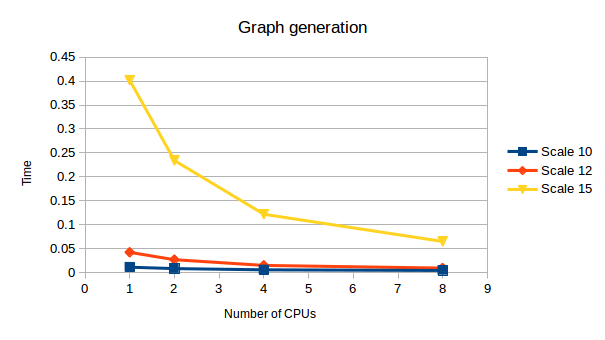
\includegraphics[width=\textwidth]{images/openmp_graphgeneration.png}
\caption{This graphs shows the graph generation time as a function of the number of CPUs used by the program}
\label{fig:graph_generation}
\end{figure}


In figure \ref{fig:openmp_scale_cpu} the TEPS can be see as a function of the CPUs used on the left and the scale on the right. Both graphs show that the amount of lines that can be traversed is almost constant.

\begin{figure}[!h]
\centering
\begin{subfigure}{.5\textwidth}
  \centering
  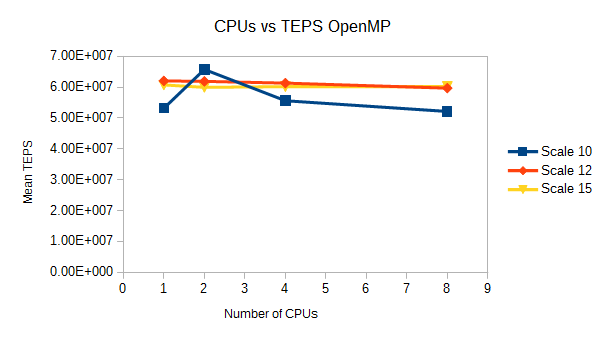
\includegraphics[width=\linewidth]{images/openmp_cpus.png}
  %\caption{A subfigure}
  %\label{fig:sub1}
\end{subfigure}%
\begin{subfigure}{.5\textwidth}
  \centering
  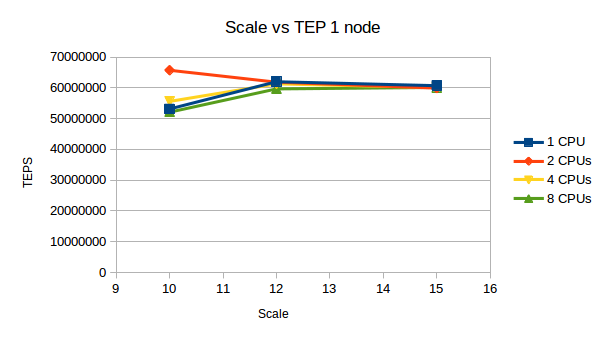
\includegraphics[width=\linewidth]{images/openmp_scale.png}
  %\caption{}
  %\label{fig:sub2}
\end{subfigure}
\caption{These figures show the effect of different of scale and the number of CPUs on the TEPS}
\label{fig:openmp_scale_cpu}
\end{figure}

\subsection{DAS-4}
In this section the results are shown of using the \texttt{graph500\_mpi\_simple} on the DAS-4. As mentioned in section[methodology], when the program is run for scales larger than 15 the program freezes. Only experiments done in next section and in section \ref{sec:openmp} have been done with validation, all other experiments have been done without.

\subsubsection{Turning validation off}
\label{sec:noval}
 Figure \ref{fig:val_vs_noval} shows the results of the amount of TEPS against the scale and the number of nodes. The figures shows that there is a difference in the number of TEPS with and without the validation. The difference can be up to 150\% in the case of scale 15 with 16 nodes. What can be noticed in figure \ref{fig:nodes_val_noval} is that the same trends are followed as the number of nodes increases. Another thing, which can be seen in figure \ref{fig:scale_val_noval}, is that the ratio of TEPS increase as the scale increases.
\begin{figure}[!h]
\centering
\begin{subfigure}{.5\textwidth}
  \centering
  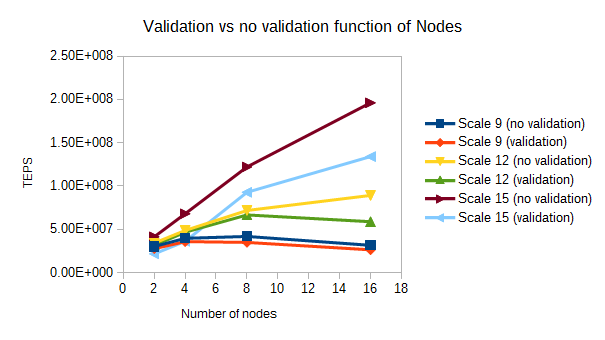
\includegraphics[width=\linewidth]{images/nodes_scale_vs_noscale.png}
  \caption{As a function of nodes}
  \label{fig:nodes_val_noval}
\end{subfigure}%
\begin{subfigure}{.5\textwidth}
  \centering
  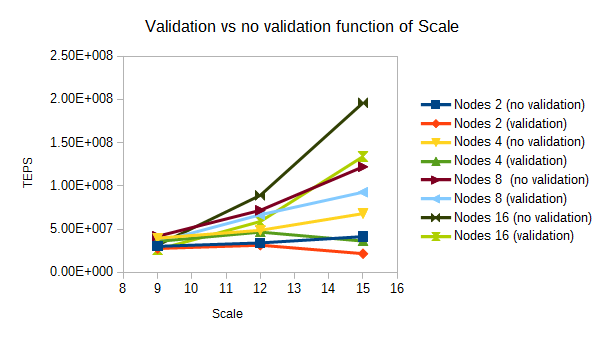
\includegraphics[width=\linewidth]{images/scale_val_vs_noval.png}
  \caption{As a function of scale}
  \label{fig:scale_val_noval}
\end{subfigure}
\caption{These figures show the effect of different of scale and the number of CPUs on the TEPS between the program with and without validation.}
\label{fig:val_vs_noval}
\end{figure}



\subsubsection{Nodes and Scale}
\label{res:nodes_scale}
In figure \ref{fig:das_no_val} shows the amount of TEPS increases as the number with the number of nodes. The larger the amount of nodes the more edges can be traversed, as seen in figure \ref{fig:scale_no_val}. This increase in TEPS can be seen up til a certain point. After this point the amount of TEPS decreases again. This tipping point can be seen in a any of the line except for the smaller scales in which the line is close to constant for any scale.
Figure \ref{fig:nodes_no_val} shows the same data but then as a function of the number of nodes. What can be seen in these figures is that the amount TEPS increases as the nodes increases per scale. These are fairly straight lines. The thing to notice is that scale 21 is performs the best of each investigate number of nodes, although for 2 and 4 nodes the amount of TEPS always about the same, independent of the scale of the problem.
One interesting thing to note is that the measurements done on scale 30 have less TEPS than the TEPS for scale 15.

\begin{figure}[!h]
\centering
\begin{subfigure}{.5\textwidth}
  \centering
  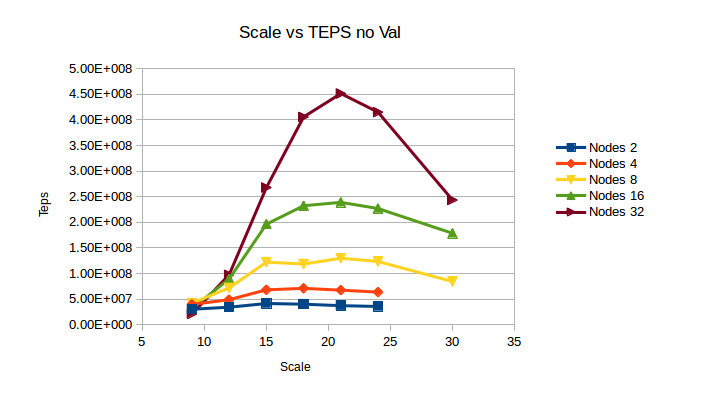
\includegraphics[width=\linewidth]{images/nodes_no_val.png}
  \caption{TEPS as a function of nodes for different scales.}
  \label{fig:nodes_no_val}
\end{subfigure}%
\begin{subfigure}{.5\textwidth}
  \centering
  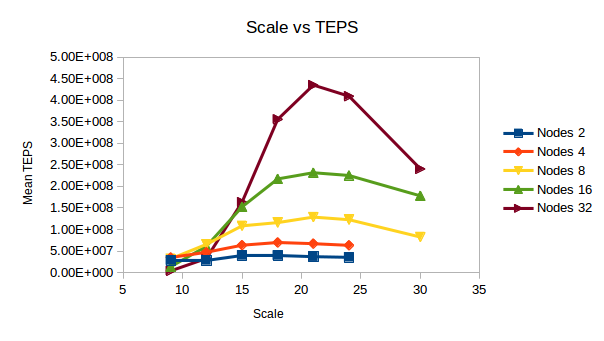
\includegraphics[width=\linewidth]{images/scale_no_val.png}
  \caption{TEPS as a function of scale for different amount of nodes.}
  \label{fig:scale_no_val}
\end{subfigure}
\caption{This figure shows the change in the amount of TEPS as a function of scale and nodes.}
\label{fig:das_no_val}
\end{figure}

\subsubsection{No InfiniBand}
The experiments on the DAS-4 have also been done run without InfiniBand. The results are similar to what has been seen previously. As before figure \ref{fig:scale_no_infini} shows an increase in TEPS as the scale increases till a certain tipping point, but unlike what has been seen in figure \ref{fig:scale_no_val} the tipping point has not been yet been reached at scale 24. Figure \ref{fig:scale_no_infini} shows that slope between scale 21 and 24 is very small, but not yet reached. The difference between the maximum value for 16 nodes from the results of section \ref{res:nodes_scale} is 6 times as large as the maximum value for the same amount of nodes from the InfiniBand experiments.
Figure \ref{fig:scale_no_infini} also shows the same trends as figure \ref{fig:scale_no_val}. 
 
\begin{figure}[!h]
\centering
\begin{subfigure}{.5\textwidth}
  \centering
  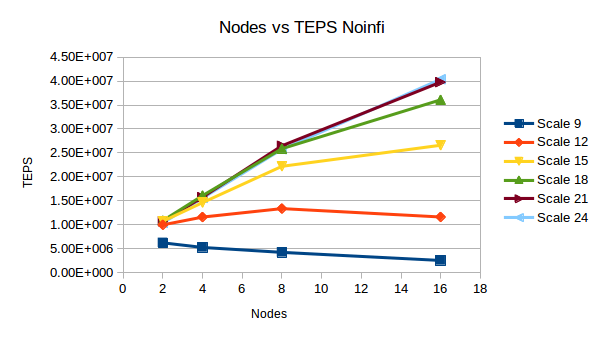
\includegraphics[width=\linewidth]{images/nodes_no_infini.png}
  \caption{TEPS as a function of nodes for different scales.}
  \label{fig:nodes_no_infini}
\end{subfigure}%
\begin{subfigure}{.5\textwidth}
  \centering
  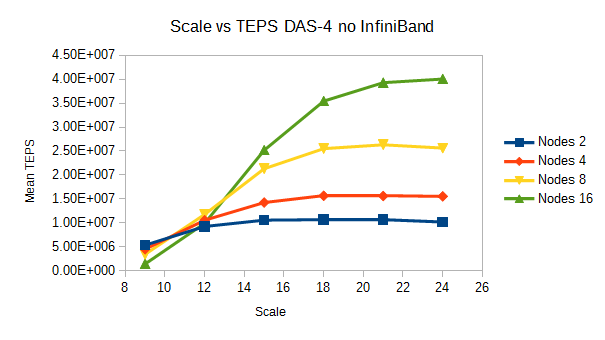
\includegraphics[width=\linewidth]{images/scale_no_infini.png}
  \caption{TEPS as a function of scale for different amount of nodes.}
  \label{fig:scale_no_infini}
\end{subfigure}
\caption{This figure shows the change in the amount of TEPS as a function of scale and nodes on the DAS-4 without using InfiniBand.}
\label{fig:das_no_infini}
\end{figure}

\subsection{OpenNebula}
The OpenNebula results can best be compared the results on the DAS-4 without InfiniBand, because the VMs on the OpenNebula also do not use Infiniband.
Looking at figure \ref{fig:das_opennebula} it is clear to see that graph is far less clear. IN both graphs you can see far more intersections and results are far less smooth than the other than the previous two graphs(figure \ref{fig:das_no_val} and \ref{fig:das_no_infini}). The difference between using 4 and 8 nodes is much less clear on the OpenNebula, four nodes sometimes has an even better performance than eight nodes.
As a whole the trends can be seen only again a few factors smaller than the results of the DAS with infiniband turned off.

\begin{figure}[!h]
\centering
\begin{subfigure}{.5\textwidth}
  \centering
  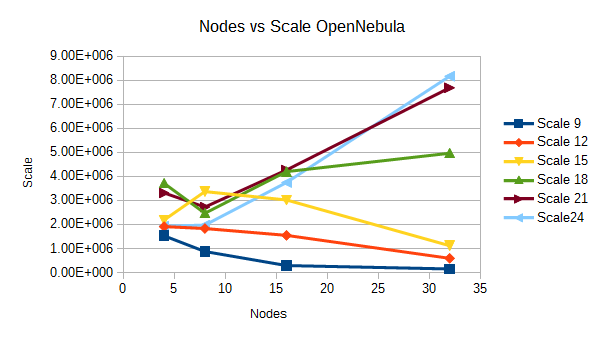
\includegraphics[width=\linewidth]{images/nodes_opennebula.png}
  \caption{TEPS as a function of nodes for different scales.}
  \label{fig:nodes_opennebula}
\end{subfigure}%
\begin{subfigure}{.5\textwidth}
  \centering
  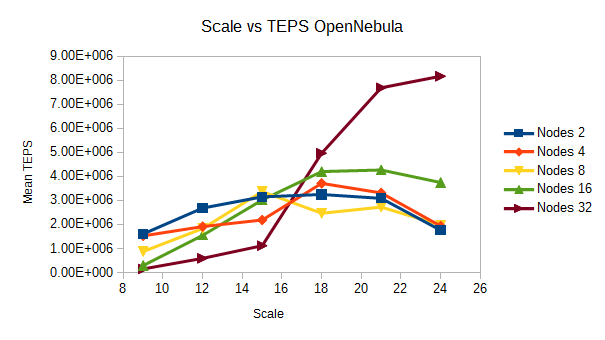
\includegraphics[width=\linewidth]{images/scale_opennebula.png}
  \caption{TEPS as a function of scale for different amount of nodes.}
  \label{fig:scale_opennebula}
\end{subfigure}
\caption{This figure shows the TEPS vs the scale and nodes for the experiments done on OpenNebula of the DAS-4.}
\label{fig:das_opennebula}
\end{figure}

\subsection{Communication}
In this section the results are shown with respect to the communication between the nodes.
\subsubsection{IMB benchmark}
On each of the systems the IMB benchmark has been done. To find the time it takes to send messages between to machines. The times which are relevant are 0, 1028 and 2048 bytes. The 0 bytes times shows the time it takes to send the finished message, 1028 bytes gives an indication of how much time it will take to send a message without a completely full buffer, and lastly the 2048 shows the time it takes to send a full buffer. The complete table is shown in Appendix [REF to appendix].
\begin{table}[!h]
\begin{tabular}{|l|l|l|l|}
\hline
Bytes & DAS-4 ($\mu sec$) & DAS-4 no InfiniBand($\mu sec$) & OpenNebula ($\mu sec$)\\ \hline
0 & 3.81 &  46.55  & 112.75  \\ \hline
1024 & 4.93 & 56.97  &  130.76 \\ \hline 
2048 & 269.74 & 5.96 & 68.36 \\ \hline
\end{tabular}
\caption{This figure shows the IMB benchmarks on the different platforms used. All times are an average of a 1000 messages sent. Only the relevant sizes have been shown.}
\label{tab:imb_bench}
\end{table}

\subsubsection{Message count}
The message count is an important number for calculate the communication time. The amount of data which is sent per message is known, but the number of messages is not known. As mentioned before in the paper by Suzumaru\cite{suzumura2011performance} an estimation for the amount of bytes which is, see equation \ref{eq:communication_size}. In figure \ref{fig:das_scale_messages} two plot can be seen. The figure shows that the estimation of data send is correct and with this the number of messages can derived by using this estimation. There is one thing to notice is that there is a factor two difference between the number of messages. 
\begin{figure}[!h]
\centering
\begin{subfigure}{.5\textwidth}
  \centering
  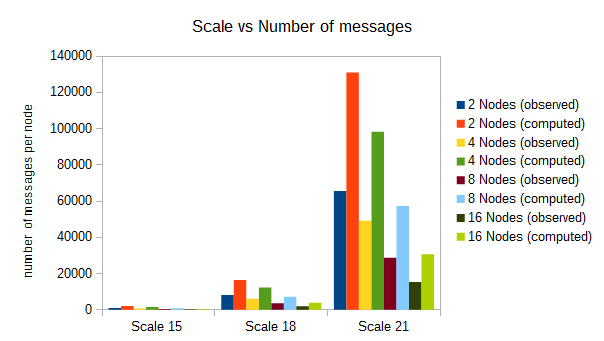
\includegraphics[width=\linewidth]{images/scale_vs_messages.png}
  \caption{The number of messages as a function of scale for different number of nodes.}
  \label{fig:scale_messages}
\end{subfigure}%
\begin{subfigure}{.5\textwidth}
  \centering
  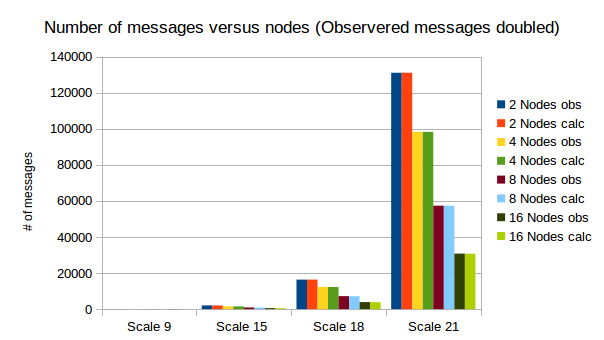
\includegraphics[width=\linewidth]{images/scale_vs_messages_doubled.png}
  \caption{The same graph as figure \ref{fig:scale_messages}, but with the observed number of messages doubled}
  \label{fig:scale_messages_doubled}
\end{subfigure}
\caption{This figure shows how the number of messages grows for 4 different scales and 2 to 16 nodes. The observed number is the number of messages sent when the buffer is full + the messages send with left overs, see section \ref{med:comm}}
\label{fig:das_scale_messages}
\end{figure}

\subsection{The model}


\section{Discussion}
\label{discussion}
In this section the results, the model, other findings and problems encountered will be discussed.

\subsection{DAS}
In the results seen in graphs \ref{fig:das_no_infini}, \ref{fig:das_no_val} following can be seen. In this figure you can see that there is a tipping point at which the number of TEPS decreases. This is unlike what can be seen in the experiments without InfiniBand and on AWS. These show a tipping point a small dip and then a steady decline as the scale increases. But the DAS experiments show a much more drastic dip in the performance after the tipping point. This is most likely because of a the network being saturated which is mentioned in the paper by angel. This paper suggest that at a certain point point the . There are 3 factors which contribute to the amount of edges that can be traversed, namely: the computation time, the communication time and the network. The maximum achievable TEPS the one that takes the maximum amount of time divided by the. The more nodes you have the more spread out the information will and the more often the information needs to be gotten from the another machine. At the start of the experiment all nodes will have a lot of nodes to process and the connection will be fine, but as the number of edges which needs to be the same nodes need to access to the same node which will clog the network.


\subsection{OpenNebula}
The results of OpenNebula the order of magnitude is much lower than what can be seen in Amazon and the DAS-4 without InifiBand even thought it is running on the same hardware as.

There were some problems with using OpenNebula. The cluster on which the latest version of OpenNebula was installed was shutdown in preparation of the new DAS-5. For this reason the older version 3.8 needed to be used. The OpenNebula marketplace does not have any images for version 3.8 anymore, which made the setup time a bit longer. Also public images available on the OpenNebula VU cluster seemed to be working out of the box. Also one thing to note is that when you are running MPI it is best not to have a firewall between the hosts. 

\subsection{Amazon}
The results seen in figure \ref{fig:c3_amazon} and \ref{fig:r3_amazon} look consistent to the thought that

Creating on demand machine on Amazon is easy, but there are some limitation

\subsection{Validation vs No Validation}
%TODO validation no validation 32 nodes or not.
AS shown in the figure \ref{fig:val_vs_noval} the ratio between TEPS as a function of nodes is a constant factor that does not exceed the 100 \% increase. This means that the estimation that is done using the no validation experiments are comparable to expected value which is given by the experiments with validation. The estimation to use the total number of edges compared to the visited actual number of edges is a good approximation and will give an answer in the right order of magnitude. 

\subsection{Reference implementation}
There were some problems with running the \texttt{graph500\_mpi\_simple} on the DAS. The first problem was that the MPI version on the DAS-4. The version used is 1.4. This MPI 1.4 is not compatible with the reference code, which uses data types defined in later versions. Because of this the texttt{workaround.h} needed to be changed. Changing the file made it possible to compile this program on the DAS-4. In the commands of this file, it is stated that this would help out with the validation and will prevent the program from hanging. This was the case for a scale up to 15. At a scale higher than 15 program would get stuck while validating the first BFS. To avoid this problem, experiments have been run with validation turned off.

\subsection{Model}
When we first thought of the model, we thought there were two factors which contribute to calculating the TEPS, namely: the computational time and the communication time. The computation time is a constant is the amount of nodes that one node can compute. The communication time is the time it takes to send all the messages. Trying to make a model with these two parameter resulted in straight lines. The computation is a linear function of the number of nodes and the communication is a function of the scale and the number of nodes, because everything is parallel and the number of and the messages which are sent are non-blocking the calculations need to be done for one node. 
The paper by Angel proposes that there is another factor which is contention on the network. What the paper suggest is that at some point the network is getting saturated. This is due to the shear amount of nodes that need to be transported over the network. This is also what can be seen in the results. As the nodes stay constant and the scale goes up there is a tipping point as mentioned in the results. After this tipping point the amount of TEPS keeps reducing. This can be explained, by looking at contention. If the scale goes up but the number of nodes stay the same the chance of contention keeps increasing. As the contention increases the network will reach is minimum value which is the maximum one link can handle. This means that it will return to a state between two nodes instead of having a parallel system of n nodes.
%TODO think about this some more.
With this new insight in mind there are multiple ways to test if this is true. One easy way to increase the buffer size. By increasing the buffer size the amount of messages that will not decrease but the timings of these messages will differ and there will not be a continues stream coming from one node only bursts.



 

\section{Conclusion}
\label{conclusion}
The project focused on finding a model to predict the performance of the a Graph 500 benchmark depending on the amount of resources.

A reasonable size of graph to process on Amazon EC2 is a scale of 30. Processing a scale 30 graph can  be done with 32 r3.large instance and takes for five hours to complete. Getting 32 instances of the r3.large on Amazon EC2 does not take a lot of effort.

The performance of the Graph 500 benchmark on the DAS-4 has been compared to the performance of the Amazon EC2. From the results we can conclude that the public cloud can be competitive with a super computer. Although there is no InfiniBand in the cloud, the latency and compute power of the machines is competitive with the DAS-4 in terms of performance.
 
A model has been created. This model is dependent on the tipping performance point. Before the point, the model is linear. After the tipping point, we approximate the model with a constant performance, which is an optimistic prediction. The parameters of this linear function are dependent on the architecture on which the benchmark is running.

\section{Future Work}
\label{future-work}
There are still experiments to be done on this subject.

A model has been made to predict the performance of the  \texttt{graph500\_mpi\_simple} on Amazon EC2 . Larger amount of nodes and higher scales should be tested. Behaviors can differ for larger scales. It has only been shown that the behavior is different for smaller scales. The same behavior as seen for scales 15 and lower might also occur for larger scales and more nodes. This needs to be investigated to refine/confirm the model largest problem scales.  

The \texttt{graph500\_mpi\_simple} could run multiple processes on one node. The program does not make use of multiple processes during the BFS. This means that if there is enough memory on the computer it would be possible to run multiple processes per node. This has already been shown in the paper by Angel et al.\cite{angel2012graph}, but it is something that has not been looked at yet.

Other implementations could be used to run on the cloud. The \texttt{graph500\_mpi\_simple} is a hardly optimized implementation. The performance can be improved by having a more optimized implementation on each node. The implementation should be hardware agnostic, if it is to run on cloud. The implementation by \cite{ueno2012highly} which do a two dimensional version of the BFS algorithm might be a good first step.
 
Also other types of cloud instances and public cloud services should be tested. Only Amazon EC2 has been during this project and only two different instance. Although these instances seemed the most relevant for this project larger instances should be tested to find out if the model still holds. Also the using the m3.large might be a good comparison to the other results. The Google cloud might also be interesting option to run the application on.

On the DAS-4 with InfiniBand showed a different behavior than all the other experiments done. This a phenomena unrelated to the Graph 500 in the cloud, but it is interesting to investigate further.

Amazon enhanced networking might be an optimization. This needs to be confirmed.


\newpage
\printbibliography

\end{document}
